%
%===============>>  Симонов Модуль 5 <<=============
%=
\setmodule{5}

%BEGIN_FOLD % ====>>_____ Занятие 1 _____<<====
\begin{class}[number=1]
	\begin{listofex}
		\item занятие 1
	\end{listofex}
\end{class}
%END_FOLD

%BEGIN_FOLD % ====>>_ Домашняя работа 1 _<<====
\begin{homework}[number=1]
	\begin{listofex}
		\item Вычислите: \quad \(\left( \dfrac{36x}{x^2-81}+\dfrac{x-9}{x+9} \right)\cdot\dfrac{x}{x+9}-\dfrac{x}{x-9}\)
		\item Рабочие прокладывают тоннель длиной \( 39 \) метров, ежедневно увеличивая норму прокладки на одно и то же число метров. Известно, что за первый день рабочие проложили \( 4 \) метра туннеля. Определите, сколько метров туннеля проложили рабочие в последний день, если вся работа была выполнена за \( 6 \) дней.
		\item Найдите площадь треугольника, основание которого равно \( 12 \), а высота --- \( 6 \).
		\item Найдите площадь равнобедренной трапеции, меньшее основание которой равно \( 15 \), боковая сторона равна \( 10 \), а высота равна \( 8 \).
	\end{listofex}
\end{homework}
%END_FOLD

%BEGIN_FOLD % ====>>_____ Занятие 2 _____<<====
\begin{class}[number=2]
	\begin{listofex}
		\item Занятие 2
	\end{listofex}
\end{class}
%END_FOLD

%BEGIN_FOLD % ====>>_ Домашняя работа 2 _<<====
\begin{homework}[number=2]
	\begin{listofex}
		\item Решите уравнения:
		\begin{tasks}
			\task \( x^2-x-2=0 \)
			\task \( -x^2+3x-2=0 \)
			\task \( 2x^2-5x+2=0 \)
			\task \( x^2-7x+12=0 \)
			\task \( 0,5x^2-3,5x+6=0 \)
			\task \( x^2-12x+11=0 \)
		\end{tasks}
		\item  Бригада маляров красит забор длиной \(270\) метров, ежедневно увеличивая норму покраски на одно и то же число метров. Известно, что за первый и последний день в сумме бригада покрасила \(90\) метров забора. Определите, сколько дней бригада маляров красила весь забор.
		\item Установите соответствие между графиками функций и формулами, которые их задают.
		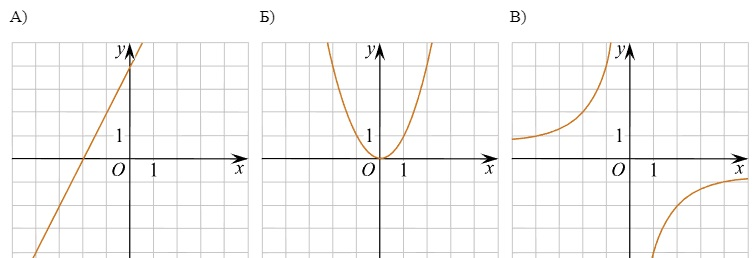
\includegraphics[align=t, width=\linewidth]{/../\picpath/SIMONOVM5H3-1}
		\begin{tasks}
			\task \(y=2x-4\)
			\task \(y=-\dfrac{4}{x}\)
			\task \(y=x^2\)
			\task \(y=2x+4\)
		\end{tasks}
	\end{listofex}
\end{homework}
%END_FOLD

%BEGIN_FOLD % ====>>_____ Занятие 3 _____<<====
\begin{class}[number=3]
	\begin{listofex}
		\item Занятие 3
	\end{listofex}
\end{class}
%END_FOLD

%BEGIN_FOLD % ====>>_ Домашняя работа 3 _<<====
\begin{homework}[number=3]
	Автомобильное колесо, как правило, представляет собой металлический диск с установленной на него резиновой шиной. Диаметр диска совпадает с диаметром внутреннего отверстия в шине.\\		
	Для маркировки автомобильных шин применяется единая система обозначений. Например, \( 195/65 R15 \) (рис. \( 1 \)). Первое число (число \( 195 \) в приведённом примере) обозначает ширину шины в миллиметрах (параметр \( B \) на рисунке 2\(  \)). Второе число (число \( 65 \) в приведённом примере) --- процентное отношение высоты боковины (параметр на рисунке \( 2 \)) к ширине шины, то есть \( 100\cdot\dfrac{H}{B} \). \\		
	Последующая буква обозначает тип конструкции шины. В данном примере буква \( R \) означает, что шина радиальная, то есть нити каркаса в боковине шины расположены вдоль радиусов колеса. На всех легковых автомобилях применяются шины радиальной конструкции.		
	За обозначением типа конструкции шины идёт число, указывающее диаметр диска колеса \( d \) в дюймах (в одном дюйме \( 25,4 \) мм). Таким образом, общий диаметр колеса \( D \) легко найти, зная диаметр диска и высоту боковины.\\		
	Возможны дополнительные маркировки, обозначающие допустимую нагрузку на шину, сезонность использования, тип дорожного покрытия и другие параметры.\\
	Завод производит легковые автомобили определённой модели и устанавливает на них колёса с шинами маркировки \( 165/70 R13 \).\\
	\begin{listofex}
		\item На сколько миллиметров увеличится диаметр колеса, если заменить колёса, установленные на заводе, колёсами с шинами маркировки \( 195/50 R15 \)?
		\item Найдите диаметр колеса автомобиля, выходящего с завода. Ответ дайте в миллиметрах.
		\item Основания трапеции равны \( 18 \) и \( 12 \), одна из боковых сторон равна \( 4\sqrt{2} \), а угол между ней и одним из оснований равен \( 135\degree \). Найдите площадь трапеции.
		\item Периметр треугольника равен \( 120 \), одна из сторон равна \( 40 \), а радиус вписанной в него окружности равен \( 7 \). Найдите площадь этого треугольника.
		\item В треугольнике \( ABC \) известно, что \( DE \) --- средняя линия. Площадь треугольника \( CDE \) равна \( 25 \). Найдите площадь треугольника \( ABC \).
	\end{listofex}
\end{homework}
%END_FOLD

%BEGIN_FOLD % ====>>_____ Занятие 4 _____<<====
\begin{class}[number=4]
	\begin{listofex}
		\item Занятие 4
	\end{listofex}
\end{class}
%END_FOLD